\colorbox{white!10!}{
    \begin{minipage}{0.2\textwidth}
       \begin{flushleft}
        
\includegraphics[width = 0.6\textwidth]{Эмблема.png}
       \end{flushleft}
    \end{minipage}
    \begin{minipage}[t]{0.7 \textwidth}
        \begin{center}
            {\huge \textsc{Красноярская Летняя Школа. Сезон $7^2 - 2$}}
            \vspace{0.25cm}
            
            { \huge \textbf{ФМТ. Тур 0.}}
        \end{center}
        \vspace{0.05cm}
    \end{minipage}
}

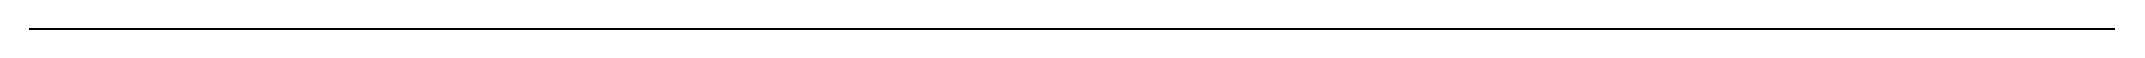
\begin{tikzpicture}
    \draw[thick] (-6.5,0)--(20,0);
\end{tikzpicture}
\begin{enumerate}
    \item Насос, мощность двигателя которого равна 25 кВт, поднимает $100\ \text{м}^3$ воду на высоту 6 м за 8 мин. Чему равен КПД установки?

    \parbox[b]{.7\textwidth}{%
    \item Определите эквивалентное сопротивление участка цепи, схема которого изображена на рисунке, если $R = 160$ Ом.   
    }\hfill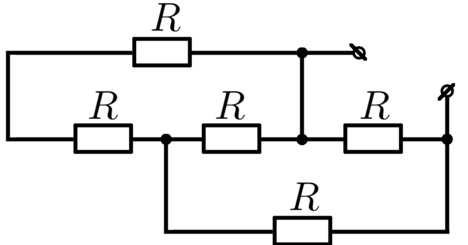
\includegraphics[width=.25\textwidth]{pictures/Tur_0.png}
\end{enumerate}